\chapter{Test de Hipótesis}


\section{Teoría de decisiones}
\label{sec:teoría_de_decisiones}

En términos generales, la teoría de decisiones estudia las acciones que puede tomar un agente en un escenario dado. En este contexto afloran de forma natural los conceptos de incertibumbre (de aspectos clave del escenario), funciones de pérdida y procedimientos de decisión. En estadística, podemos identificar al menos los siguientes problemas de decisión.


\begin{itemize}
	\item \textbf{Estimación}: Decidir el valor apropiado para un parámetro desconocido usando datos $X$ y un distribución condicional $P_\theta$
	\item \textbf{Test}: Decidir la hipótesis correcta usando datos $X\sim P_\theta$
	\begin{align}
		H_0: P_\theta\in\cP_0\\
		H_1: P_\theta\not\in\cP_0
	\end{align}
	\item \textbf{Ranking}: Elaborar una lista ordenada de ítems, por ejemplo, productos evaluados por una muestra de la población, resultados de eventos deportivos o juegos online. 
	\item \textbf{Predicción}: Estimar/decidir el valor de una variable dependiente en base a observaciones de observaciones pasadas. 
\end{itemize}

Como se puede apreciar, la teoría de decisiones presenta un contexto general para abordar una gran cantidad de situaciones. A continuación se describen los elementos básicos de un problema de decisión, en donde, con fines ilustrativos, ponemos como ejemplo su contraparte en el problema de estimación.

\begin{itemize}
	\item $\Theta = \{\theta\}$ es el espacio de estado, donde la cantidad $\theta$ es el \textit{estado del mundo}. En el problema de estimación, donde convenientemente se ha usado la misma notación, $\theta$ es el parámetro del modelo
	\item $\cA=\{a\}$ es el espacio de acciones, donde $a$ es la acción a tomar por el estadístico. En estimación, podemos usar una notación simplificada y considerar acción $a$  como la elección del valor $a$ para el parámetro $\theta$. 
	\item $L(\theta,a)$ es la función de pérdida asociada a tomar la decisión $a$ cuando el estado es $\theta$; nótese que $L:\Theta\times\cA\rightarrow\R$. En el caso de estimación, usualmente consideramos la pérdida cuadrática:
	\begin{equation}
		L(\theta,a) = (\theta-a)^2.
	\end{equation}
\end{itemize}

\begin{example}(Inversión bajo incertidumbre)
	Consideremos los estados $\Theta = \{\theta_1,\theta_2\}$, donde $\theta_1$ quiere decir mercado sano y $\theta_2$ quiere decir mercado no sano. Se debe elegir una estrategia de inversión del siguiente conjunto $\cA=\{a_1,a_2,a_3,a_4,a_5,a_6\}$, en base a la siguiente función de pérdida $L(\theta,a)$.
	\begin{table}[ht]
		\centering
		\begin{tabular}{c|c|c|c|c|c}
			$L(\theta,a)$   & $a_1$ & $a_2$ & $a_3$ & $a_4$ & $a_5$ \\
			\hline
			$\theta_1$ & -4   & -4   & -1   & 2    & 4    \\
			$\theta_2$  & 4    & 0    & -1   & -6   & -4
		\end{tabular}
	\end{table} 

	Notemos que \begin{itemize}
		\item $a_1, a_2$ son buenos  cuando $\theta=\theta_1$
		\item $a_4,a_5$ son buenos cuando $\theta=\theta_2$
		\item $a_3$ es medianamente bueno (pérdida negativa) siempre
	\end{itemize}
	entonces, ¿cómo elegimos la acción?
\end{example}

Además de los elementos básicos del problema de decisión (estado, acciones y pérdida), en el enfoque estadístico de la teoría de decisiones existen los siguientes elementos:
\begin{itemize}
	\item $X\sim P_\theta$ es la variable aleatoria, la cual define la distribución condicional, el espacio muestral, la densidad, etc. 
	\item $\delta(X)$ es el procedimiento de la decisión, es decir, el mapa que asocia una observación $X=x$ con la acción $a$:
	\begin{equation}
		\delta(\cdot):\cX\rightarrow\cA.
	\end{equation}
	\item $\cD=\{\delta:\cX\rightarrow\cA\}$ es el espacio de decisiones
	\item $R(\theta,\delta)$ es el riesgo asociado a $\delta$ y $\theta$, el cual está definido como el valor esperado de la pérdida incurrida al tomar la acción $\delta(X)$ cuando el parámetro es $\theta$. Es decir, 
	\begin{equation}
	 	R(\theta,\delta) = \Et{L(\theta,\delta(X))}.
	 \end{equation} 
\end{itemize}


\begin{example}
	Volviendo al contexto del problema de estimación, consideremos el uso de una VA $X\sim\cN(\theta,1), \theta\in\R$, para encontrar el valor del parámetro $\theta$. En el contexto de teoría estadística de decisiones, el espacio de posibles acciones es precisamente en espacio de parámetros, es decir, 
	\begin{equation}
		\cA = \Theta = \R.
	\end{equation}
	Elegimos además la pérdida cuadrática, $L(\theta,\thetahat(X)) = (\theta-\thetahat(X))^2$, asociada a estimar $\theta$ mediante $\thetahat(X)$. Consideremos que el espacio de acciones está dado por versiones escaladas de la observación $X$, es decir, 
	\begin{equation}
		\cA = \{cX, c\in[0,1]\}.
	\end{equation}
	Con esta forma del estimador, podemos calcular el riesgo asociado mediante  
	\begin{equation}
		R(\theta,\thetahat)= \Et{(\thetahat(X)-\theta)^2} = \Vt{\thetahat(X)} + \Et{\thetahat(X)-\theta}^2 = c^2 + (c-1)^2\theta^2
	\end{equation}
	¿Qué valor de $c$ sugiere elegir?
\end{example}

\begin{remark}
    La elección del parámetro $c$ en el ejemplo anterior no es trivial. Denotando el procedimiento $\delta_c$ (que asigna la acción $a=cX$), notemos que $\delta_1$ domina cualquier procedimiento $\delta_c,c\geq 1$, lo que quiere decir que el procedimiento $\delta_c$ es \textbf{inadmisible} para $c\in[1,\infty]$. Para el resto del intervalo, ningún procedimiento  $\delta_c,c\in [0,1]$ domina a otro, lo que quiere decir que son   \textbf{admisibles}.   
\end{remark}

\section{Intuición en un test de hipótesis} 
\label{sec:int_hipótesis}

El objetivo del análisis estadístico es obtener conclusiones razonables mediante el uso de observaciones, como también aseveraciones precisas sobre la incertidumbre asociada a dichas conclusiones. De forma ilustrativa, consideremos el siguiente escenario hipotético.

En base a estudios preliminares, se sabe que los pesos de los recién nacidos (RN) en Santiago, Chile, distribuyen aproximadamente normal con promedio 3000gr y desviación estándar de 500gr. Creemos que los RNs en Osorno pesan, en promedio, más que los RNs en Santiago. Nos gustaría formalmente aceptar o rechazar esta hipótesis. 

Intuitivamente, una forma de evaluar esta hipótesis es tomar una muestra de RNs en Osorno, calcular su peso promedio y verificar si éste es \textit{significativamente mayor} que 3000gr. Asumamos que hemos tenido acceso al peso de 50 RNs nacidos en Osorno, los cuales exhiben un preso promedio de 3200gr. ¿Podemos entonces concluir directamente y decir que efectivamente los RNs de Osorno pesan más que los de Santiago?  Si bien esta es una posibilidad, una postura más escéptica podría argumentar que el obtener una población de 50 RNs con peso promedio de 3200gr es perfectamente plausible de una población de RNs distribuidos de acuerdo a $\cN(3000,500^2)$. Entonces, ¿cómo justificamos la plausibilidad de este resultado?

Para esto distingamos entre las dos hipótesis: 

\begin{itemize}
	\item $H_1$: Los RNs en Osorno pesan en promedio más de 3000gr (esta es la hipótesis alternativa)
	\item $H_0$: Los RNs en Osorno pesan en promedio 3000gr (esta es la hipótesis nula)
\end{itemize}

Para decidir cuál es verdadera, trataremos de \emph{falsificar} $H_0$. La forma de hacer esto es calcular la probabilidad de obtener el resultado observado bajo el supuesto que $H_0$ es cierta. En este caso, sabemos que una muestra 
\begin{equation}
	X = X_1,\ldots,X_{50}\sim\cN(3000,500^2),
\end{equation}
tiene una media que está distribuida de acuerdo a la siguiente densidad 
\begin{equation}
	\bar{X} = \frac{1}{50} \sum_{i=1}^{50} X_i \sim \cN(3000,500^2/50).
\end{equation}
Entonces, cuál es la probabilidad de que la la distribución anterior haya generado una muestra $\bar{X}\geq3200$? Para calcular esto, construyamos el \textbf{pivote} (también conocido como $z$-test)
\begin{equation}
	z = \frac{\bar{X}-3000}{500/\sqrt{50}}\sim\cN(0,1),
\end{equation}
con el cual podemos realizar el cálculo:
\begin{equation}
	\Prob{\bar{X}\geq 3200} = \Prob{z = \frac{\bar{X}-3000}{500/\sqrt{50}}\geq 2\sqrt{2}} = 0.0023388674905235884,
\end{equation}
donde el valor de esta probabilidad puede ser calculado usando la función\footnote{Acrónimo de \textit{cumulative denstiy function}.} \texttt{cdf} de SciPy mediante la siguiente instrucción. 
\begin{lstlisting}[language=Python]
	from scipy.stats import norm
	import numpy as np
	print(1-norm.cdf(2*np.sqrt(2)))
\end{lstlisting}
Concluimos entonces que la probabilidad de que una muestra de 50 RNs exhiban un promedio de peso mayor o igual a 3200gr, bajo el supuesto que $H_0$ es cierta, es del orden del 0.23\%. 

Nos referiremos a esta probabilidad como \textbf{p-valor}, el cual nos dice cuán verosímil es obtener la observación dada bajo el supuesto de que la hipótesis nula $H_0$ es cierta. Mientras más pequeño es el p-valor, entonces más fuerte es la evidencia en contra de $H_0$. Entonces nos encontramos ante dos posibles explicaciones: 
\begin{itemize}
 	\item $H_0$ es falsa
 	\item hemos obtenido un resultado que solo ocurre una de cada 434 veces. 
 \end{itemize} 

Nos referiremos a significancia del test $\alpha$ al umbral para el p-valor en el cual se rechaza el test. En general, este umbral es del 1\% o del 5\%, sin embargo esto depende de la aplicación en cuestión. Por ejemplo, si estamos considerando la evaluación de la vacuna para Covid-19 debemos ser muy estrictos. Entonces necesariamente nuestro nivel de significancia debe ser muy bajo, lo que quiere decir que la hipótesis nula requiere mucha evidencia en su contra para ser rechazada. 

En un test de hipótesis hay dos tipos de errores posibles: El error de Tipo I en el cual $H_0$ es rechazada a pesar de que es verdadera, y el error de Tipo II donde $H_0$ no es rechazada a pesar de que es falsa (lo cual diremos que tiene probabilidad $\beta$). Los tipos de errores se definen mediante la siguiente Tabla y Figura 

\vspace{1em}
\begin{center}
	\begin{tabular}{c|cc}
			  & $H_0$ es cierto & $H_0$ no es cierto  \\
			\hline
			se rechaza $H_0$  & \emph{false positive} o error Tipo I ($\alpha$) & \emph{true positive} ($1-\beta$)    \\
			no se rechaza $H_0$  & \emph{true negative} ($1-\alpha$) & \emph{false negative} o error Tipo II ($\beta$)
	\end{tabular}
\end{center}

\begin{figure}[h]
    \centering
    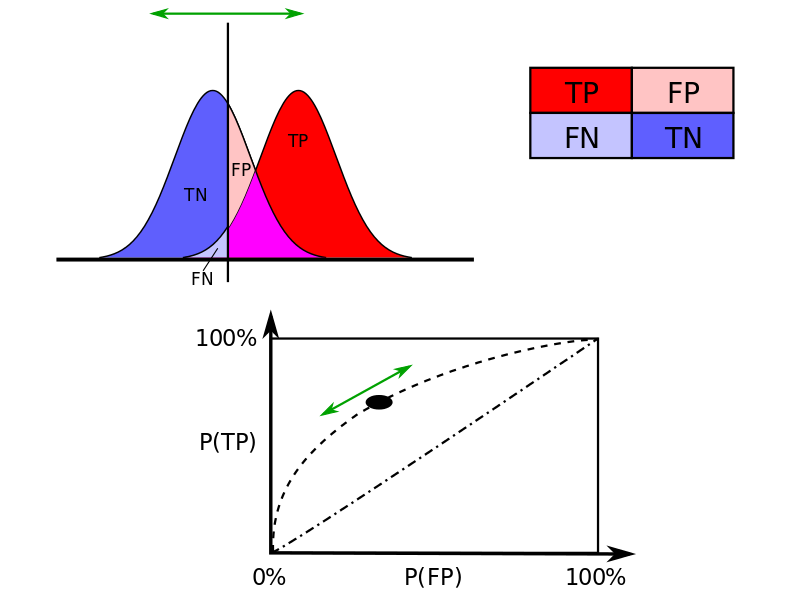
\includegraphics[trim = {0 300pt 0 0}, clip, width=0.75\textwidth]{img/ROC_curves.svg.png}
    \caption{Ilustración de tipos de errores (adaptada de Sharpr - Own work, CC BY-SA 3.0, https://commons.wikimedia.org/w/index.php?curid=44059691)}
    \label{fig:tipos_de_errore_TDH}
\end{figure}

Volviendo a nuestro ejemplo de los recién nacidos, el p-valor del test es del orden de 0.0023, lo cual, si consideramos una significancia del $\alpha=0.01=1\%$, resulta en el rechazo de $H_0$. Decimos entonces que \textbf{ hay suficiente evidencia para rechazar $H_0$ al 1\%}  (falsificación de la hipótesis nula), o bien que \textbf{ rechazamos la hipótesis nula $H_0$ al 1\%} (doble negación). Por el contrario, en el caso que el p-valor fuese mayor que el nivel de significancia del test, entonces no rechazamos $H_0$ y simplemente decimos que \textbf{ la evidencia para rechazar $H_0$ no es significativa al 1\%}. Es importante notar que solo podemos \textbf{no rechazar} la hipótesis nula, mas no confirmarla.


\begin{tcolorbox}[title=Test de Hipótesis]
En resumen,  un test de hipótesis consta de los siguientes pasos: 

\begin{enumerate}
	\item Proponer una hipótesis alternativa $H_1$
	\item Construir una hipótesis nula $H_0$ (básicamente lo contrario de $H_1$)
	\item Recolectar datos
	\item Calcular el pivote (un estadístico de prueba) usando los datos
	\item Calcular el p-valor para el pivote
	\item Comparar el p-valor con la significancia estadística. 
	\item Rechazar si corresponde
\end{enumerate}
\textbf{ADVERTENCIA: } Existe la mala costumbre de usar métodos de Test de Hipótesis, incluso cuando no corresponde. Comúnmente, usar estimación e intervalos de confianza son mejores herramientas. Sólo se debe usar Test de Hipótesis cuando se tiene una hipótesis bien definida.
\end{tcolorbox}

\textbf{Sobre p-valor y región crítica.}
Otra forma de cuantificar la evidencia en contra de $H_0$ es mediante la identificación de una región crítica, es decir, un subconjunto de $\cX$ en donde, de tomar valores la observación (o el estadístico), su p-valor estaría por debajo del nivel de significancia y consecuentemente $H_0$ se rechazaría. En el ejemplo anterior, este puede ser calculado usando la función de SciPy \texttt{ppf}\footnote{Acrónimo para \emph{percent point function}.}. Considerando una significancia del 1\% podemos ejecutar
\begin{lstlisting}[language=Python]
	from scipy.stats import norm
	print(norm.ppf(0.99))
\end{lstlisting}
lo cual nos da una región crítica $[2.326,\infty)$, la cual contiene a nuestro umbral $2\sqrt{2} = 2.82$; concluimos de igual forma y rechazamos $H_0$ al 1\%. 

\begin{figure}[ht]
    \centering
    \includegraphics[scale=0.7]{img/Region_critica.png}
    \caption{La región crítica son aquellos valores que tienen una probabilidad menor al nivel de significancia, en este caso, el 1 $\%$}
    \label{fig:region_critica}
\end{figure}
\begin{remark}
Un hipótesis de la forma $\left \{ \theta=\theta_0\right \}$ se dice hipótesis simple. Una hipótesis de la forma $\theta > \theta_0$ o $\theta < \theta_0$ se dice hipótesis compuesta. Un test de la forma :
 $$
 H_0: \theta=\theta_0 \text{ versus } H_1:\theta \not = \theta_0
 $$
se dice bilateral, y un test de la forma: 
$$
H_0: \theta \leq \theta_0 \text{ versus } H_1:\theta > \theta_0
$$
se dice unilateral. 

Los tests bilaterales son los más comunes.  Notemos que en la Figura \ref{fig:region_critica} no ocupamos las dos colas de la figura, pues hicimos un test unilateral. Si hubiésemos hecho un test bilateral (\emph{"Los recién nacidos tienen una media distinta a 3000"}), habríamos ocupado las dos colas de la normal. 
\end{remark}

\todo[inline]{Falta discusión sobre test simétricos y asimétricos: gráfico ilustrando el uso de p-valor, pivote, significancia y región crítica.}


\section{Rechazo, potencia y nivel} 
\label{sec:def_hipótesis}

Formalmente, frente a dos hipótesis generales denotadas por 
\begin{align}
	H_0&: \theta\in\Theta_0\\
	H_1&: \theta\in\Theta_1,
\end{align}
definiremos el problema del test de hipótesis como la búsqueda de una función
\begin{equation}
	\phi:\cX\rightarrow \{0,1\},
\end{equation}
donde:
\begin{itemize}
	\item Si $\phi(x)=0$ entonces aceptamos $H_0$ (no rechazamos $H_0$).
	\item Si $\phi(x)=1$ entonces rechazamos $H_0$, lo cual implícitamente acepta $H_1$. 
\end{itemize}
En teoría de decisiones, diríamos que $\phi$ es una regla de decisión. 

A continuación, revisamos definiciones que serán de utilidad para analizar y construir tests. 

\begin{definition}[Región crítica de un test]
	La región crítica o región de rechazo de un test de hipótesis $\phi$ se define como 
	\begin{equation}
		R_\phi = \{x\in\cX | \phi(x)=1\} = \phi^{-1}(1).
	\end{equation}
	
\end{definition}



\begin{definition}[Función de probabilidad de rechazo]
Para un test $\phi$ y cualquier parámetro $\theta\in\Theta$ podemos definir la probabilidad de rechazo mediante
\begin{equation}
 	\alpha_\phi(\theta) = \Probt{\phi(x)=1} = \Probt{x\in R_\phi}, \forall\theta\in\Theta,
 \end{equation}
donde nos gustaría entonces que $\alpha\approx 0$ si $\theta\in\Theta_0$ es cierto y que $\alpha\approx 1$ si $\theta\in\Theta_1$. Luego, usaremos esta función para evaluar la calidad del test.
\end{definition}

\begin{definition}[Potencia de un test]
En el caso que $H_1$ sea cierta, es decir, $\theta\in\Theta_1$, podemos definir la potencia del test como la probabilidad rechazar $H_0$ cuando $H_1$ es efectivamente cierta ($\theta\in\Theta_1$). Es decir,
\begin{equation}
 	\pi_\phi(\theta) = \Prob{\text{rechazar } H_0 | H_1 \text{ es cierta}}  = \Probtu{\phi(x)=1}.
 \end{equation}
 \end{definition}
Nos gustaría entonces minimizar $\alpha(\theta)$ cuando $H_0$ y maximizar $\alpha(\theta)$ cuando $H_1$, lo cual es equivalente a minimizar la probabilidad de cometer errores de Tipo I y II respectivamente. 


\begin{example}[Un test absurdo]
	Existen tests absurdos, por ejemplo $\phi(x) = 0,\forall x\in\cX$. Este test tiene $\alpha(\theta)=0$ cuando $H_0$ (lo cual es bueno), pero también tiene potencia nula, es decir, incluso si $H_1$, no rechaza a $H_0$. 
 \end{example} 
 En general, consideramos más importante prevenir un error de tipo I que uno de tipo II. Es decir, nos protegemos ante el rechazo de $H_0$ cuando es cierta. 

 \begin{definition}[Nivel de un test]
 Decimos que un test es de nivel $\alpha\in[0,1]$ si 
\begin{equation}
 		\alpha_\phi(\theta)\leq\alpha, \forall \theta\in\Theta_0,
 	\end{equation}
 	equivalentemente, $\sup_{\theta\in\Theta_0}\alpha_\phi(\theta)\leq\alpha$. Además, denotamos por $T_\alpha$ la clase de todos los tests de nivel $\alpha$. 
 \end{definition}
 Dentro de esta clase, la cual nos restringe únicamente a los test que tienen probabilidad de rechazo acotada superiormente por $\alpha$  para $\theta\in\Theta_0$ (probabilidad de cometer error tipo I), podemos buscar el test de mayor potencia (probabilidad de rechazar $H_0$ cuando $H_1$ es cierta). Caracterizamos este test mediante: 

 \begin{definition}[Test uniformemente más potente, UMP]
 	Diremos que $\phi^\star$ es un test UMP (de nivel $\alpha$)  si 
 	\begin{equation}
 		\pi_{\phi^\star}(\theta)\geq \pi_{\phi}(\theta), \forall\theta\in\Theta_1.
 	\end{equation}
 	
 \end{definition}


\section{Test de Neyman-Pearson} 
\label{sub:test_de_neyman_pearson}
Consideremos el siguiente problema de test de dos hipótesis simples. 
\begin{equation}
	H_0:\theta\in\Theta_0=\{\theta_0\}\quad \text{v.s.}\quad H_1:\theta\in\Theta_1=\{\theta_1\},
\end{equation}
donde por una notación más simple escribiremos simplemente 
\begin{equation}
	H_0:\theta =\theta_0\quad \text{v.s.}\quad H_1:\theta = \theta_1,		
\end{equation}
y asumiremos que $\familiaparametrica=\{P_{\theta_0},P_{\theta_1}\}$ con densidades respectivamente dadas por $p_0(x) = p_{\theta_0}(x)$ y $p_1(x) = p_{\theta_1}(x)$.

Denotamos además la región crítica (donde se rechaza $H_0$) mediante
\begin{equation}
	\label{eq:R_NR}
	R^* = \{x\in\cX | p_1(x) \geq k p_0(x)\},
\end{equation}
donde $k\in\R_+$ es una constante a determinar. 

Podemos entonces definir el test $\phi^*$ como el test que tiene el conjunto $R^*$ como región de rechazo, es decir, 
\begin{equation}
	\phi^*(x) = 1 \Leftrightarrow x\in R^*.
\end{equation}

Finalmente, determinaremos la constante $k$ de tal manera de que 
\begin{equation}
	\alpha_{\phi^\star}(\theta_0) = \mathbb{P}_{\theta_0}(x\in R^*) = \alpha,\ \alpha\in[0,1], 
\end{equation}
donde, por definición, $\phi^\star\in T_\alpha$. Consecuentemente, de acuerdo al siguiente lema, $\phi^\star$ es el test UMP en $T_\alpha$.

\begin{lemma}[Neyman-Pearson]
	Consideremos un test de hipótesis de la forma 
	\begin{equation}
		H_0:\theta =\theta_0\quad \text{v.s.}\quad H_1:\theta = \theta_1
	\end{equation}
	con probabilidad de rechazo dada por
	\begin{equation}
			\alpha = \mathbb{P}(p_1(X)\geq k p_0(X)).
		\end{equation}
	Entonces, este test es el UMP de nivel $\alpha$.
\end{lemma}

\begin{proof}
	Denotemos $\phi^*$ el test de Neyman-Pearson y $R^*$ su región critica, por definición, $\phi^*\in T_\alpha$. Además, consideremos otro test $\phi\in T_\alpha$ con su propia región crítica $R$. Recordemos que  la probabilidad de los datos estén en la región R es ($\forall \theta$)
	\begin{equation}
		\Probt{R} = \int_R p_\theta(x)\dx.
	\end{equation}
	Luego, podemos escribir 
	\begin{align}
		\Probt{R} &= \Probt{R\cap R^*} + \Probt{R\cap \bar{R}^*}\\
		\Probt{R^*} &= \Probt{R^*\cap R} + \Probt{R^*\cap \bar{R}},
	\end{align}
	restando y evaluando para $\theta=\theta_1$, tenemos
	\begin{align}
	\Probtu{R^*} - \Probtu{R} 	&=  \Probtu{R^*\cap \bar{R}} - \Probtu{R\cap \bar{R}^*}\nonumber \\
								&=  \int_{R^*\cap \bar{R}} p_{\theta_1}(x)\dx - \int_{R\cap \bar{R}^*} p_{\theta_1}(x)\dx\nonumber\\
									&\geq  k\int_{R^*\cap \bar{R}} p_{\theta_0}(x)\dx - k\int_{R\cap \bar{R}^*} p_{\theta_0}(x)\dx \quad[\text{pues } p_1\geq k p_0 \text{ en } R^*]\nonumber\\
									&= k\left( \Probtz{R^*\cap \bar{R}} - \Probtz{R\cap \bar{R}^*}\right)\nonumber \\
									&= k\left( \underbrace{\Probtz{R^*}}_{=\alpha} - \underbrace{\Probtz{R}}_{\leq\alpha}\right) \quad[\text{primera igualdad de este desarrollo}]\nonumber\\
									&\geq 0
	\end{align}
	Hemos probado que $\Probtu{R^*} \geq \Probtu{R}$. Es decir, si $\theta = \theta_1$ entonces $x\in\R^*$ tiene mayor probabilidad que cualquier otra región $R$. Consecuentemente,  el test que tiene a $R^*$ por región crítica es el test UMP.

	
\end{proof}


\begin{example}
	Sea $X_1,\ldots, X_n$ iid $\ber{\theta}, \theta\in\{\theta_0,\theta_1\}$: 
	\begin{equation}
		H_0:\theta =\theta_0\quad \text{v.s.}\quad H_1:\theta = \theta_1.
	\end{equation} 
	Asumamos que $\theta_1>\theta_0$ y expresemos las densidades de cada hipótesis como 
	\begin{equation}
		p_i(x) = \theta_i^{\sum x_j}(1-\theta_i)^{n-\sum x_j},\ i=0,1.
	\end{equation}
	Para rechazar $H_0$ según el test de Neyman-Pearson, es decir, $x\in R^*$ de acuerdo a la ecuación \eqref{eq:R_NR}, el test requiere: 
	\begin{equation}
		\label{eq:ejemplo:NR}
		\frac{p_1(x)}{p_0(x)} = \frac{\theta_1^{\sum x_j}(1-\theta_1)^{n-\sum x_j}}{\theta_0^{\sum x_j}(1-\theta_0)^{n-\sum x_j}} = \left(\frac{1-\theta_1}{1-\theta_0}\right)^n\left(\frac{\theta_1(1-\theta_0)}{\theta_0(1-\theta_1)}\right)^{\sum x_j}\geq k. 
	\end{equation}
	Como $\theta_1\geq\theta_0$, la expresión anterior es monótona en  $\sum x_j$, consecuentemente, $\sum x_j$ debe ser lo suficientemente grande para rechazar $H_0$. 
	
	Para calcular el valor de $k$ dado un $\alpha$, tenemos que resolver $\Probtz{x\in R^*} = \alpha$, para lo cual notemos que la ecuación \eqref{eq:ejemplo:NR} es equivalente a 
	\begin{align}
	 	\left(\frac{1-\theta_1}{1-\theta_0}\right)^n\left(\frac{\theta_1(1-\theta_0)}{\theta_0(1-\theta_1)}\right)^{\sum x_j}\geq k 
	 	& \Leftrightarrow 
	 	\left(\frac{\theta_1(1-\theta_0)}{\theta_0(1-\theta_1)}\right)^{\sum x_j}\geq k \left(\frac{1-\theta_0}{1-\theta_1}\right)^n\\
	 	& \Leftrightarrow 
	 	\sum x_j \loga{\frac{\theta_1(1-\theta_0)}{\theta_0(1-\theta_1)}}\geq n \loga{k \left(\frac{1-\theta_0}{1-\theta_1}\right)} \nonumber\\
	 	& \Leftrightarrow 
	 	\sum x_j \geq \frac{n \loga{k \left(\frac{1-\theta_0}{1-\theta_1}\right)}}{\loga{\frac{\theta_1(1-\theta_0)}{\theta_0(1-\theta_1)}}} = k'. \nonumber
	 \end{align} 
	 Finalmente, como $\sum x_j$ es binomial, podemos resolver directamente para $k'$ (y consecuentemente para $k$). La región crítica  está definida mediante 
	 \begin{equation}
	     R^* = \left\{(x_1,\ldots,x_1) \text{ t.q. } \sum x_j\geq k'\right\}.
	 \end{equation}
\end{example}


\section{Test de Wald} 
\label{sub:test_de_wald}

Este test nos permite evaluar si un parámetro $\theta$ toma no un valor $\theta_0$ dado. Consideremos un parámetro escalar y $\thetahat$ un estimador asintóticamente normal, es decir, 
\begin{equation}
	\frac{\thetahat - \theta_0}{\ee} \sim \cN(0,1),
\end{equation}
cuando el número de observaciones tiende a infinito y $\ee=\sqrt{\V{\thetahat}}$ es conocido como el \emph{error estándar} y puede ser calculado muestralmente o desde $p_{\theta_0}$. Entonces, el test de Wald de tamaño $\alpha$ para las hipótesis 
	\begin{equation}
		H_0:\theta =\theta_0\quad \text{v.s.}\quad H_1:\theta \neq \theta_0,
	\end{equation}
indica rechazar $H_0$ cuando el pivote $W=\frac{\thetahat - \theta_0}{\ee}$ cumple con 
\begin{equation}
	|W|\geq z_{\alpha/2},
\end{equation}
donde $z_{\alpha/2}=\Phi(1-\alpha/2)$, es decir, $\Prob{Z\geq z_{\alpha/2}}=\alpha/2,\ Z\sim\cN(0,1)$. 

\begin{remark}
	Notemos que, asintóticamente, el nivel del test de Wald de tamaño  $\alpha$, es $\alpha$. En efecto, 
\begin{equation}
	\Probtz{|W|\geq z_{\alpha/2}} = \Probtz{\left|\frac{\thetahat - \theta_0}{\ee}\right|\geq z_{\alpha/2}} \rightarrow  \Probtz{|Z|\geq z_{\alpha/2}} = \alpha
\end{equation}
donde, hemos usado que $Z\sim\cN(0,1)$.
\end{remark}


\begin{example}
 Consideremos dos conjuntos de VAs $X_1,\ldots,X_n$ y $Y_1,\ldots,Y_m$, con medias respectivas $\mu_1$ y $\mu_2$. Se requiere evaluar las hipótesis
 	\begin{equation}
		H_0:\mu_x =\mu_y \quad \text{v.s.}\quad H_1:\mu_x \neq \mu_y,
	\end{equation}
	lo cual está dentro del alcance del test de Wald denotando $\delta = \mu_x - \mu_y$ e identificando las hipótesis
	 	\begin{equation}
		H_0:\delta =0 \quad \text{v.s.}\quad H_1:\delta \neq 0.
	\end{equation}
Utilicemos el estimador no-paramétrico `plug in' de $\delta$ dado por  $\hat{\delta} = \bar{X}-\bar{Y} = \frac{1}{n}\sum_{i=1}^n x_i - \frac{1}{m}\sum_{i=1}^m y_i$. Además, la varianza de este estimador está dada por $v = \frac{1}{n}s_x^2 + \frac{1}{m}s_y^2$ (por el CLT), con lo que el  estadístico de Wald es
\begin{equation}
	W = \frac{\hat{\delta}-0}{\ee} = \frac{\bar{X}-\bar{Y}}{\sqrt{\frac{1}{n}s_x^2 + \frac{1}{m}s_y^2}},
\end{equation}
y rechazamos rechazamos $H_0$ si
\begin{equation}
	|\bar{X}-\bar{Y}| \geq z_{\alpha/2} \sqrt{\frac{1}{n}s_x^2 + \frac{1}{m}s_y^2},
\end{equation}
donde recordemos que el lado derecho decae como $1/\sqrt{n}$.
\end{example}

\begin{remark}
Notemos que el test de Wald de tamaño $\alpha$ rechaza $H_0:\theta=\theta_0$ (v.s. $H_1:\theta\neq\theta_0$) si y solo si 
\begin{equation}
	\theta_0 \notin (\thetahat - \ee z_{\alpha/2},\thetahat + \ee z_{\alpha/2}),
\end{equation}
es decir, realizar el test de Wald es equivalente a calcular el $\alpha$ intervalo de confianza para el parámetro $\theta_0$ asumiendo normalidad.
\end{remark}


\section{Test de razón de verosimilitud} 
\label{sub:test_de_RV}

Consideremos un caso más general que los anteriores, donde al menos una de las hipótesis es compuesta, es decir, especifican que el parámetro pertenece a un conjunto en vez de tomar un valor puntual. Es decir, 
\begin{equation}
		H_0:\theta \in\Theta_0\quad \text{v.s.}\quad H_1:\theta \notin\Theta_0.
	\end{equation}
El test de razón de verosimilitud (TRV) indica que se debe rechazar $H_0$ si 
\begin{equation}
	\label{eq:lambda_TRV}
	\lambda(x_1,\ldots,x_n) = \frac{\sup_{\theta\in\Theta_0}L(\theta)}{\sup_{\theta\in\Theta}L(\theta)}
							= \frac{L(\thetahat_0)}{L(\thetahat)}\leq C,
\end{equation}
donde $\thetahat$ es el EMV y $\thetahat_0$ es el EMV restringido a $\{\theta\in\Theta_0\}$. Claramente, la región de rechazo está dada por 
\begin{equation}
	R^* = \{x\in\cX|\lambda(x)\leq C\}.
\end{equation}
\begin{remark}
	Para el caso de hipótesis simples, es decir, $\Theta = \{\theta_0,\theta_1\}$ y $\Theta_0 = \{\theta_0\}$, entonces el TRV coincide con el test de Neyman-Pearson (TNP). Al igual que en el TNP, en el TRV fijamos $C$ en función del un nivel deseado $\alpha$. 
\end{remark}


\begin{remark}
	Notemos que podemos escribir la expresión en la ecuación \eqref{eq:lambda_TRV} como 
	\begin{equation}
		\lambda(x_1,\ldots,x_n) =  \ind_{\thetahat\in\Theta_0} + \ind_{\thetahat\not\in\Theta_0} \frac{\sup_{\theta\in\Theta_0}L(\theta)}{\sup_{\theta\not\in\Theta_0}L(\theta)}
	\end{equation}
	donde el segundo término (de activarse) es estrictamente menor que 1, con lo que el TRV puede enunciarse en función del estadístico 
	\begin{equation}
		\tilde{\lambda}(x_1,\ldots,x_n) = \frac{\sup_{\theta\in\Theta_0}L(\theta)}{\sup_{\theta\not\in\Theta_0}L(\theta)} \leq \tilde{k}.
	\end{equation}
\end{remark}


\begin{example}[TRV Bernoulli]
	Sea $X_1,\ldots,X_n\sim\ber{\theta}$ iid, se quiere resolver
	\begin{equation}
		H_0:\theta \leq\theta_0\quad \text{v.s.}\quad H_1:\theta >\theta_0,
	\end{equation}
donde $\theta_0$ es conocido y sabemos que $p_\theta(x) = \theta^{n\bar{x}}(1-\theta)^{n(1-\bar{x})}$. En la notación de la definición anterior del TRV, podemos identificar
\begin{equation}
	\Theta_0 = [0,\theta_0] \quad \& \quad \Theta_1 = (\theta_0, 1]
\end{equation}
calculamos el EMV (restricto e irrestricto) mediante 
\begin{align}
	\thetahat &= \bar{x}\quad \text{irrestricto}\\
	\thetahat_0 &= \bar{x} \quad \text{si } \bar{x}\in\Theta_0,\ \theta_0 \text{ si no.}
\end{align}
podemos escribir esta última expresión como $\thetahat_0 = \bar{x} \ind_{\bar{x}\in\Theta_0} + \theta_0\ind_{\bar{x}\notin\Theta_0}$, entonces

\begin{align}
	\lambda(x) &= \frac{L(\thetahat_0)}{L(\thetahat)}\\ 
				&= \frac{L(\bar{x})}{L(\bar{x})} \ind_{\bar{x}\in\Theta_0} + \frac{L(\theta_0)}{L(\bar{x})} \ind_{\bar{x}\notin\Theta_0} \\
				&= \ind_{\bar{x}\in\Theta_0} + \ind_{\bar{x}\notin\Theta_0} \left(\frac{\theta_0}{\bar{x}}\right)^{n\bar{x}}\left(\frac{1-\theta_0}{1-\bar{x}}\right)^{n(1-\bar{x})}
\end{align}
\begin{figure}[ht]
    \centering
    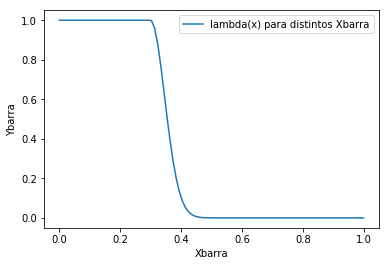
\includegraphics[scale=0.7]{img/LKratio.png}
    \caption{$\lambda(x)$ en función de $\bar{x}$}
    \label{fig:lk_ratio}
\end{figure}
Donde ahora rechazaremos si $\lambda(x)\leq C$, pero, ¿cómo elegimos $C$?

Al igual que en TNP, podemos imponer que el test sea de nivel $\alpha$, es decir, 
\begin{equation}
 	\sup_{\theta\in\Theta_0} \Probt{\lambda(x)\leq C} = \alpha
 \end{equation} 
 donde recordemos que $\lambda(x)$ es una función decreciente de $\bar{x}$, por lo que la condición $\lambda(x)\leq C$ puede expresarse como $\bar{x}\geq C'$, para algún $C'$. Esta expresión dependerá de $C'$, que es función de $C$, de $\theta_0$ y de $\alpha$; despejamos para $C$.
 
 \end{example} 
 
 \begin{remark}
     En general, los umbrales para los tests de hipótesis son fijados en función del nivel deseado. Consecuentemente, podemos escribir $k=k(\alpha)$ y $C=C(\alpha)$ en TNP y TRV respectivamente. 
 \end{remark}

% \section{Test Chi cuadrado} 


 \section{Test de Kolmogorov-Smirnov} 
\label{sub:test_KS}

Ahora consideramos otro enfoque, basado en una estrategia muy distinta, al problema de test de hipótesis anterior para distribuciones no paramétricas. Buscamos determinar si la distribución $F$ de una VA es igual a una distribución de referencia $F_0$ o no, es decir: 
	\begin{equation}
		H_0:F=F_0\quad \text{v.s.}\quad H_1:F\neq F_0.
	\end{equation}
Consideremos además la distribución empírica dada por 
\begin{equation}
	F_n(x) = \frac{1}{n}\sum_{i=1}^n\ind_{x_j\leq x}, 
\end{equation}
la cual realmente es una distribución (discontinua y  constante por tramos). 

Sabemos que, debido a la ley de los grandes números, 
\begin{equation}
	F_n(x)\to \E{\ind_{X\leq x}} = \Prob{X\leq x} =  F(x),
\end{equation}
además, por el teorema de Glivenko-Cantelli, tenemos 
\begin{equation}
	\sup_x|F_n(x)-F(x)| \to 0 \quad\text{c.s.}
\end{equation}
Lo anterior nos permite definir el estadístico  $D_n = \sup_x|F_n(x)-F_0(x)|$ y la región crítica
\begin{equation}
	R = \{x|D_n\geq k_\alpha\},
\end{equation}
donde $k_\alpha$ se elige imponiendo $\Probtz{D_n\geq  k_\alpha}=\alpha$.

\begin{remark}
El test de  Kolmogorov-Smirnoff sirve tanto para verificar si una VA sigue una distribución dada o si bien dos distribuciones siguen la misma distribución (desconocida).
\end{remark}

 \section{Test de Wilcoxon} 
\label{sub:test_Wilc}

Este es otro testo no paramétrico para verificar si dos VAs siguen la misma distribución. Consideremos las observaciones 
\begin{equation}
	X_1,\ldots,X_n\sim F,\quad Y_1,\ldots,Y_n\sim G,
\end{equation}
donde $F$ y $G$ son dos distribuciones, de las cuales solo sabemos que son continuas. 

Consideremos el siguiente problema de test de hipótesis: 
	\begin{equation}
		H_0:F=G\quad \text{v.s.}\quad H_1:F\neq G.
	\end{equation}
El test de Wilcoxon se enfoca en este escenario pero solo es sensible a diferentes \emph{localizaciones}, es decir, si $G$ es una versión desplazada de $F$.

Antes de ver el test de Wilcoxon, notemos que si nos interesase detectar estas desviaciones, entonces podríamos considerar un test que rechace $H_0$ si $|\bar{X} - \bar{Y}|\geq K$. Esto  es exactamente lo que hace el TRV en el problema 
	\begin{equation}
		H_0:\mu =  \eta \quad \text{v.s.}\quad H_1:\mu\neq \eta,
	\end{equation}
cuando $X\sim\cN(\mu,\sigma^2)$,  $Y\sim\cN(\eta,\sigma^2)$.

Sin embargo, en el caso general (cuando no sabemos nada de $F$) obtener la ley de $|\bar{X} - \bar{Y}|$ bajo $H_0$ no es trivial, lo cual es necesario para $\Probtz{|\bar{X} - \bar{Y}|\geq K} = \alpha$. En esta situación, el test de Wilcoxon propone considerar la siguiente observación conjunta 
\begin{equation}
	(z_1,\ldots,z_{m+n}) = (x_1,\ldots,x_n,y_1,\ldots,y_m),
\end{equation}
para luego considerar la secuencia ordenada de valores $z_i$ dados por 
\begin{equation}
	\min_i\{z_i\} = z_{(1)}\leq z_{(2)}\leq\cdots\leq z_{(n+m)} = \max_i\{z_i\}.
\end{equation}

Ahora podemos definir el concepto de \emph{rango} como la posición en el orden anterior, es decir, donde el rango de $z_{(1)}$ es 1, el rango de $z_{(2)}$ es dos  y así sucesivamente. 

\todo[inline]{dibujo de bolas negras y blancas.}

Denotando el rango de $x_i$ como $R_i$, podemos construir el estadístico
\begin{equation}
 	W = \sum_{i=1}^{n}R_i,
 \end{equation} 
esta cantidad debe intuitivamente interpretarse como el promedio de los rangos (es decir de la posiciones) que toman las observaciones de la variable $X$, por rechazamos $H_0$ si $W$ es muy pequeño o muy grande, es decir, si las muestras de $X$ no quedan \emph{mezcladas} con las de $Y$. 

 Esto es posible por que la distribución de $W$ bajo $H_0$ puede ser calculada y de hecho no depende de $F$, esto es porque (bajo $H_0$) los elementos de $z_i$ son iid, con lo que todas las posible permutaciones del los valores $z_i$ tienen la misma probabilidad dada por $\binom{n+m}{n}$.

 \begin{remark}[¿Cómo obtenemos la región crítica $R$ para este test?]
 	Podemos proceder de forma iterativa: Asumimos $H_0$, consideramos $R=\emptyset$ y agregamos las configuraciones de bolitas que tienen el menor y mayor valor de $W$, luego seguimos con las siguientes configuraciones hasta acumular una probabilidad $\Probtz{W\in\R} = \alpha$.
 \end{remark}
 
 \section{Test de Hipótesis Bayesiano}
 Hasta ahora sólo hemos visto los distintos test de hipótesis desde una perspectiva frecuentista. En todos estos test, había una relación asimétrica entre dos hipótesis: la hipótesis nula $H_0$ y la hipótesis alternativa $H_1$. Un proceso de desición se lleva acabo, y luego, en base a los datos observados, la hipótesis nula se va a rechazar a favor de $H_1$, o se aceptará. \\
 En el test de hipótesis Bayesiano, puede haber más de dos hipótesis en consideración, y no deben tener, necesariamente, una relación asimétrica.
 Para simplificar el análisis, consideremos dos hipótesis: $H_1$ y $H_2$.\\
 Sabemos que en algún momento tendremos datos $X$, sin embargo, aún no los tenemos. Nos interesa calcular las distribuciones posteriores $P(H_1|X)$ y $P(H_2|X)$. Usando Bayes: 
 $$
 P(H_1|X)=\dfrac{P(X|H_1)P(H_1)}{P(X)} \text{ ; }
 P(H_2|X)=1-P(H_1|X).
 $$
Por probabilidades totales: 
$$
P(X)=P(X|H_1)P(H_1)+P(X|H_2)P(H_2).
$$
\begin{example}
    Consideremos un lanzamiento de una moneda, y las hipótesis: $H_1=$"La moneda está cargada" ($\theta=\frac{1}{2}$) y $H_2$="La moneda no está cargada". Entonces, si $\theta$ es la probabilidad de que salga cara (C):
    $$
    P(\theta|H_1)=1_{\theta=0.5}
    $$
    Esto es una distribución a priori. Por otra parte, la hipótesis 2 es la que indica que la moneda está cargada. Consideremos que si la moneda está cargada, $\theta$ puede valer $1/3$ o $2/3$ de forma igualmente probable: 
     $$
    P(\theta|H_2)= 0.5 *1_{\theta=\frac{1}{3}} + 0.5* 1_{\theta=\frac{2}{3}}
    $$
    Por último, necesitamos las probabilidades $P(H_1)$ y $P(H_2)$. Consideremos (como se suele hacer) que $P(H_1)=P(H_2)=0.5$. Supongamos que al lanzar la moneda obtenemos la secuencia: CCSCSC. Entonces: 
    $$
    P(X|H_1)=  \binom{6}{4} (\dfrac{1}{2})^{4}(\dfrac{1}{2})^{2} =  \binom{6}{4} 0.0156 
    $$
    $$
    P(X|H_2) = P(X|\theta=1/3)P(\theta=1/3)+  P(X|\theta=2/3)P(\theta=2/3) =\binom{6}{4} 0.0137 
    $$
    Con los dos cálculos anteriores: 
    $$
    P(X)= \binom{6}{4} 0.0156 P(H_1) + \binom{6}{4} 0.0137 P(H_2) = \binom{6}{4} 0.01465
    $$
    Entonces: 
    $$
    P(H_1|X)=\dfrac{ \binom{6}{4} 0.0156 P(H_1)}{\binom{6}{4} 0.01465}  = 0.53
    $$
    Luego pasamos de $P(H_1)=0.5$ a $P(H_1|X)=0.53$, es decir, actualizamos nuestras creencias y ahora pensamos que es más probable que la moneda no esté cargada.
\end{example}
 
 En el test bayesiano, el ratio entre las verosimilitudes se llama \textbf{factor de bayes}.
